% !TeX root = ../main.tex

\section{Problem Definition}
    \frame{\sectionpage}

    \begin{frame}{Seat Planning with Social Distancing}
      \begin{itemize}
      \item Group type $\mathcal{M} = \{1, \ldots, M\}$.
      \item Row $\mathcal{N} = \{1, \ldots, N\}$.
      \item The number of seats in row $j$: $S_j, j \in \mathcal{N}$.
      \item $\delta$ seat(s) as the social distancing.
      \item Let $n_i = i + \delta$ denote the new size of group type $i$ for each $i \in \mathcal{M}$.
      \item Let $L_j = S_j + \delta$ denote the length of row $j$ for each $j \in \mathcal{N}$.
      \end{itemize}
      
      \begin{figure}[ht]
        \centering
        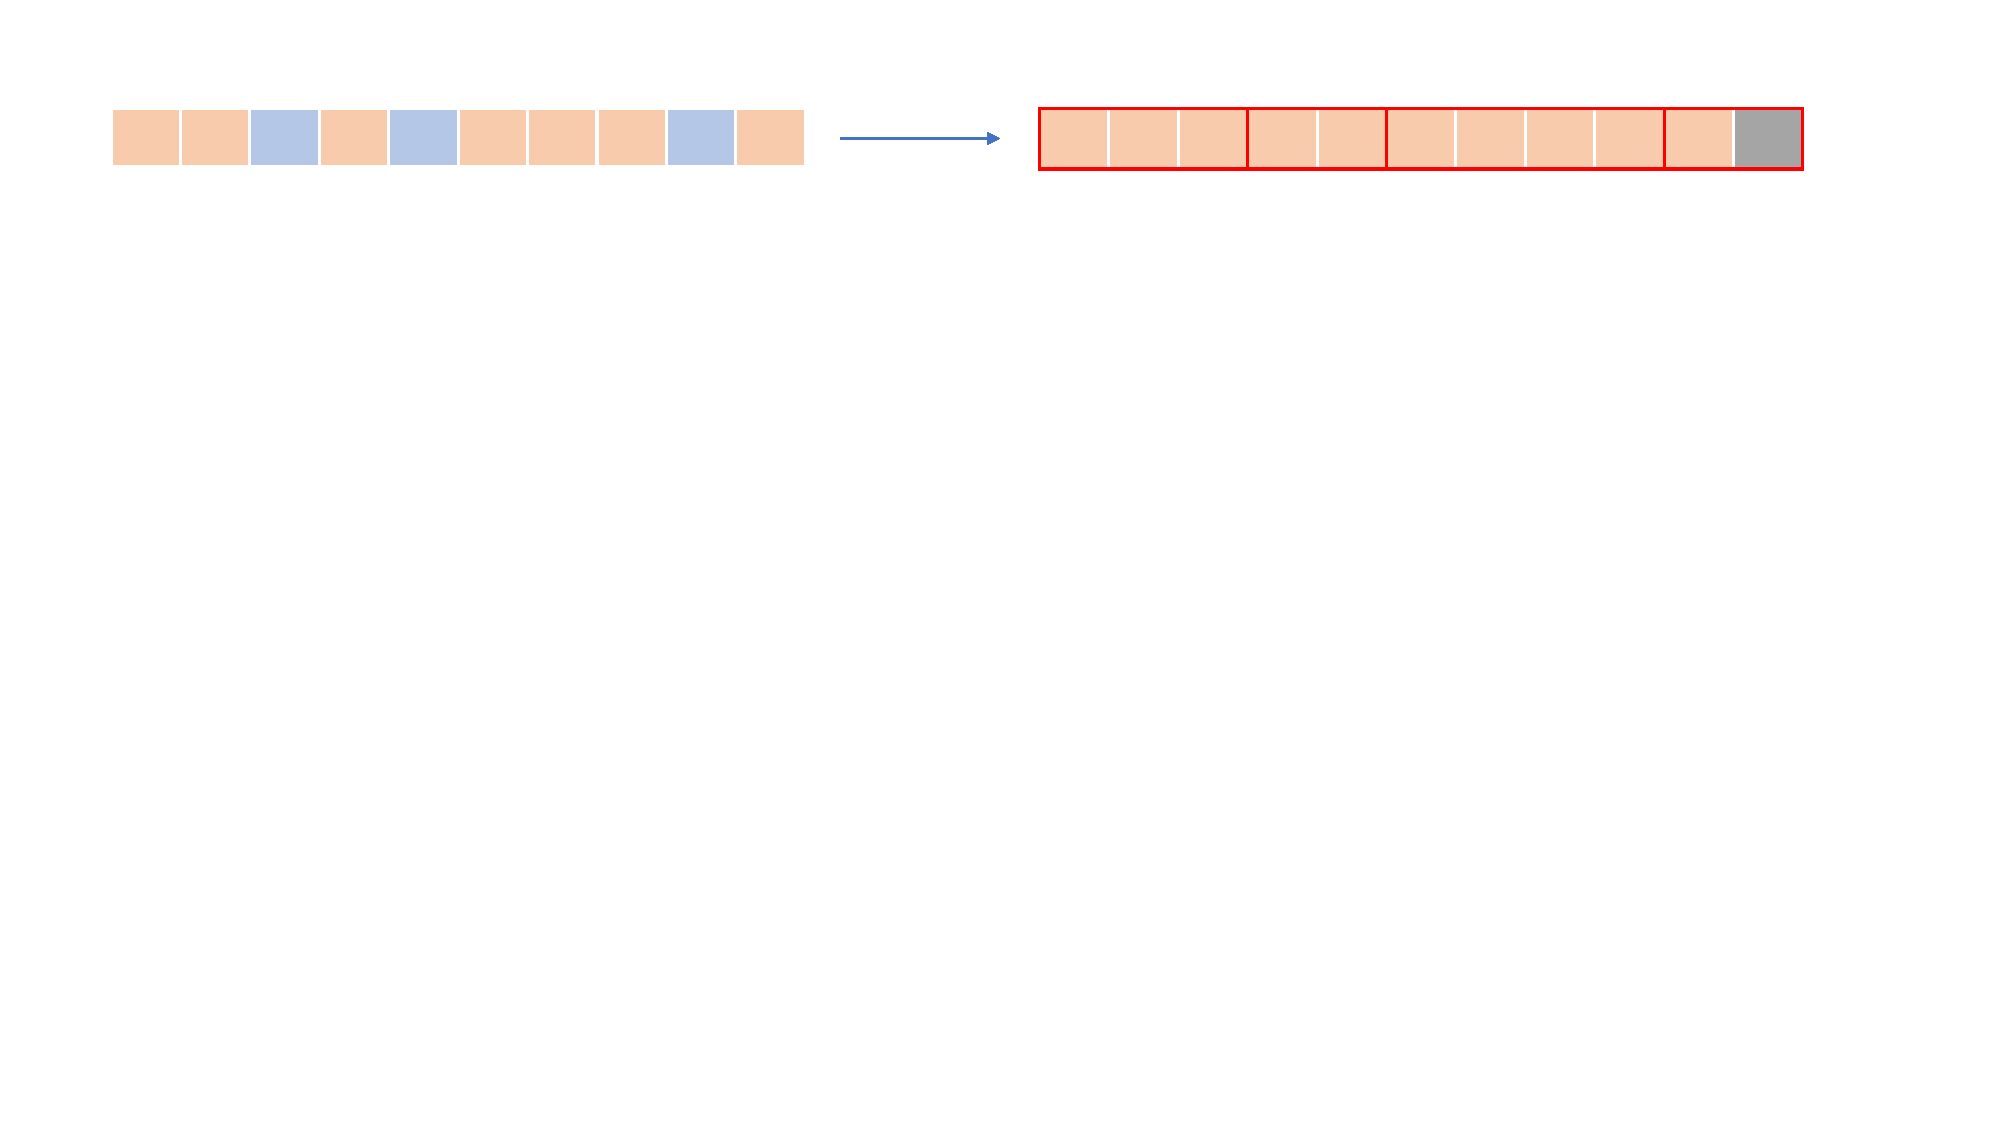
\includegraphics[width = 0.8\textwidth]{./images/dummy_seat.pdf}
        \caption{Problem Conversion with One Seat as Social Distancing}
    \end{figure}
    \end{frame}

  \begin{frame}{Basic Concepts}
    \begin{itemize}
      \item Pattern refers to the seat planning for one row.
      \item For each pattern $k$, $\alpha_k, \beta_k$ indicate the number of groups and the left seats, respectively.
      \item Denote by $\alpha_k \delta + \beta_k - \delta$ the loss for pattern k, $l(k)$. The loss represents the number of people lost compared to the situation without social distancing.
      \item Let $I_1$ be the set of patterns with the minimal loss. We call the patterns from $I_1$ are the largest. The patterns with zero left seat are called full patterns.
      \item Suppose there are $n$ groups in a row, for ease of brevity, we use a descending form $P_{k} = (t_1, t_2, \ldots, t_n)$ to denote pattern $k$, where $t_h$ is the new group size, $h = 1,\ldots, n$.
    \end{itemize}
  \end{frame}

  \begin{frame}{Example}
    \begin{itemize}
      \item Suppose the social distancing is one seat and there are four types of groups. Then the new sizes of groups are $2, 3, 4, 5$, respectively. 
      % \item The demand for each group type is $[10, 12, 9, 8]_d$. 
      \item The length of one row is $L = 21$.
      \item Then these patterns, $(5, 5, 5, 5), (5, 4, 4, 4, 4),(5, 5, 5, 3, 3)$, belong to $I_1$.
      \item Pattern $(5, 5, 5, 5)$ is not full because there is one left seat.
    \end{itemize}
  \end{frame}

  \begin{frame}{Loss of The Largest Patterns}
    \begin{itemize}
      \item[-] The largest pattern can be obtained by the greedy way: select the maximal group size, $n_{M}$, as many times as possible, then $L = n_{M} \cdot q + r, 0 \leq r < n_{M}$, $r$ is the number of empty seats. 
      \item[-] When $r > \delta$, these seats can be occupied by the group type $(r-\delta)$; when $r \leq \delta$, leave these seats empty.
      \item[*] Loss of the largest pattern: $q \delta -\delta + f(r)$, where $f(r) =0$ if $r > \delta$; $f(r) = r$ if $r \leq \delta$.
      \item[*] For a seat layout, $\{S_1, S_2, \ldots, S_{N}\}$, the minimal total loss: $\sum_{j} (\lfloor \frac{S_j+\delta}{n_{M}} \rfloor -\delta + f((S_j + \delta) \mod n_{M}))$. The maximal number of people assigned: $\sum_{j} (S_j - \lfloor \frac{S_j+\delta}{n_{M}} \rfloor + \delta - f((S_j +\delta)\mod n_{M}))$.
    \end{itemize}
  \end{frame}
  
  \begin{frame}{Dynamic Seat Assignment Problem}
    \centering
    Dynamic seat assignment can be characterized by DP:
    $$V_{t}(\mathbf{L}) = \mathbb{E}_{i \sim p}\left[\max_{\substack{j \in \mathcal{N}: \\ L_j \geqslant {n}_{i}}}\left\{V_{t+1}\left(\mathbf{L}- n_{i}\mathbf{e}_j^{\intercal} \right)+ i, V_{t+1}(\mathbf{L})\right\}\right]$$
    $$V_{T+1}(\mathbf{L}) = 0,$$

    \begin{itemize}
      \item[-] $L^{r}_{j}$: the number of remaining seats in row $j$.
      \item[-] $\mathbf{L} = (L^{r}_1, L^{r}_2, \ldots, L^{r}_{N})$: remaining capacity. 
      \item[-] $p_i$: the probability of an arrival of group type $i$.
    \end{itemize}
\end{frame}